% Progress Report Document
\documentclass[progress]{cmpreport}
\makeatletter
\input{t1pcr.fd}
\makeatother
\setlength{\footnotesep}{3ex}
\title{\Codex: A Website and Progressive Web App in Node.js \& React for table-top role-playing games}
\author{Christopher Alastair Irvine}
\registration{100036248}
\supervisor{Dr Katharina Huber}
\ccode{CMP-6013Y}
\summary{This document is the Progress Report for Codex}
\acknowledgements{
	I would like to thank Dr Katharina Huber for taking on the supervision of this project, 
	and guiding me towards greatness. Additionally I would like to thank Wizards of the Coast 
	for their generosity and kindness in allowing the use of their Intellectual Property for this project.
}
\usepackage{rotating}
\usepackage{amsmath}
\usepackage{lscape}
\usepackage{hhline}
\usepackage{caption}
\usepackage{makecell}
\newcommand{\ueacmp}{UEA School of Computing Sciences}
\newcommand{\WotC}{Wizards of the Coast}
\newcommand{\dnd}{D\&D}
\newcommand{\sem}{Software Engineering Model}
\newcommand{\sems}{Software Engineering Models}
\newcommand{\Codex}{\textsc{Codex}}
\newcommand{\AgileSolo}{\emph{Agile Solo}}
% EOF Preamble and Macros
	
% BOF Document
\begin{document}
	% BOF Introduction
	\section{Introduction} \label{sec:intro}
	% Introduction to the project:
	Dungeons and Dragons (\dnd) is a popular table-top role-playing game which (for the purposes of \Codex) is based on the following principles. \dnd \ is random and the game cannot survive without a \emph{Dungeon Master} (DM). For a glossary of \dnd \ terms and concepts, please see Appendix \ref{app:example}. Terms and Concepts introduced in Appendix \ref{app:example} will be referred to throughout this document. A typical \dnd \ set up can been seen in Figure \ref{fig:DnDEquipmentExample}
	
	\begin{figure}
		\begin{subfigure}{0.5\textwidth}
			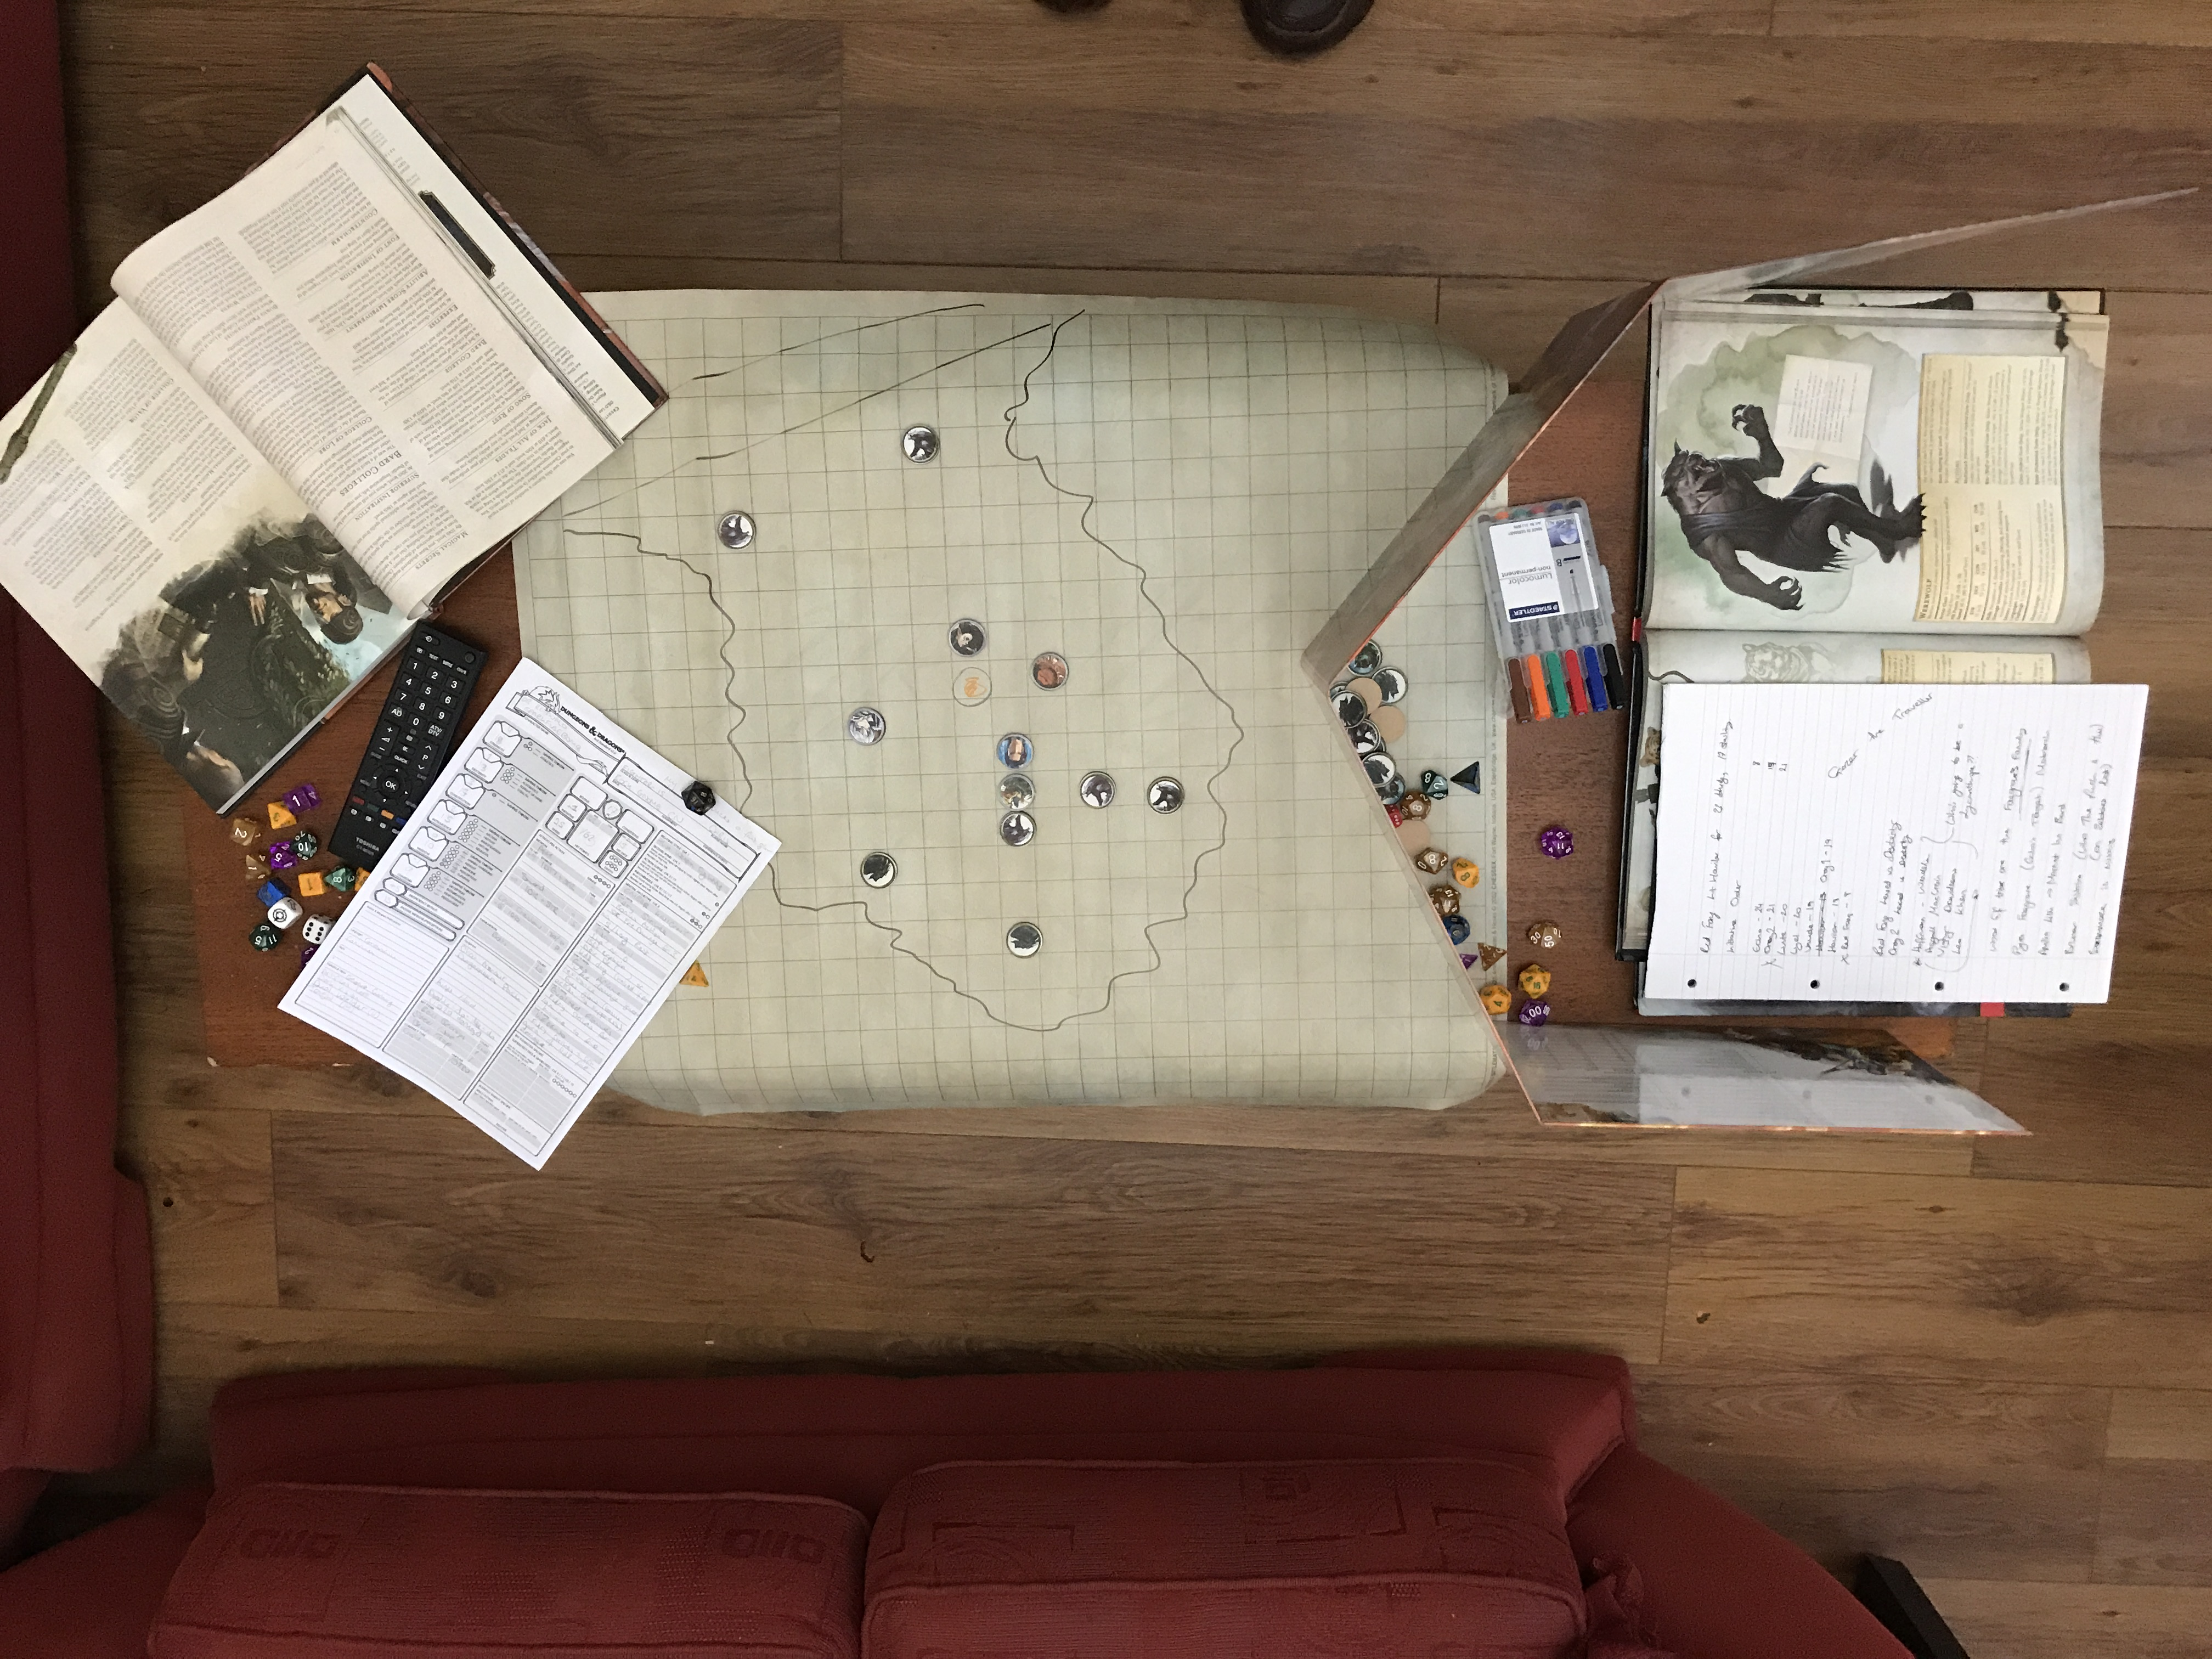
\includegraphics[width=1\linewidth, height=5cm, angle=180]{DnD_Live.jpg}
			\label{DnDLive}
		\end{subfigure}
		\begin{subfigure}{0.5\textwidth}
			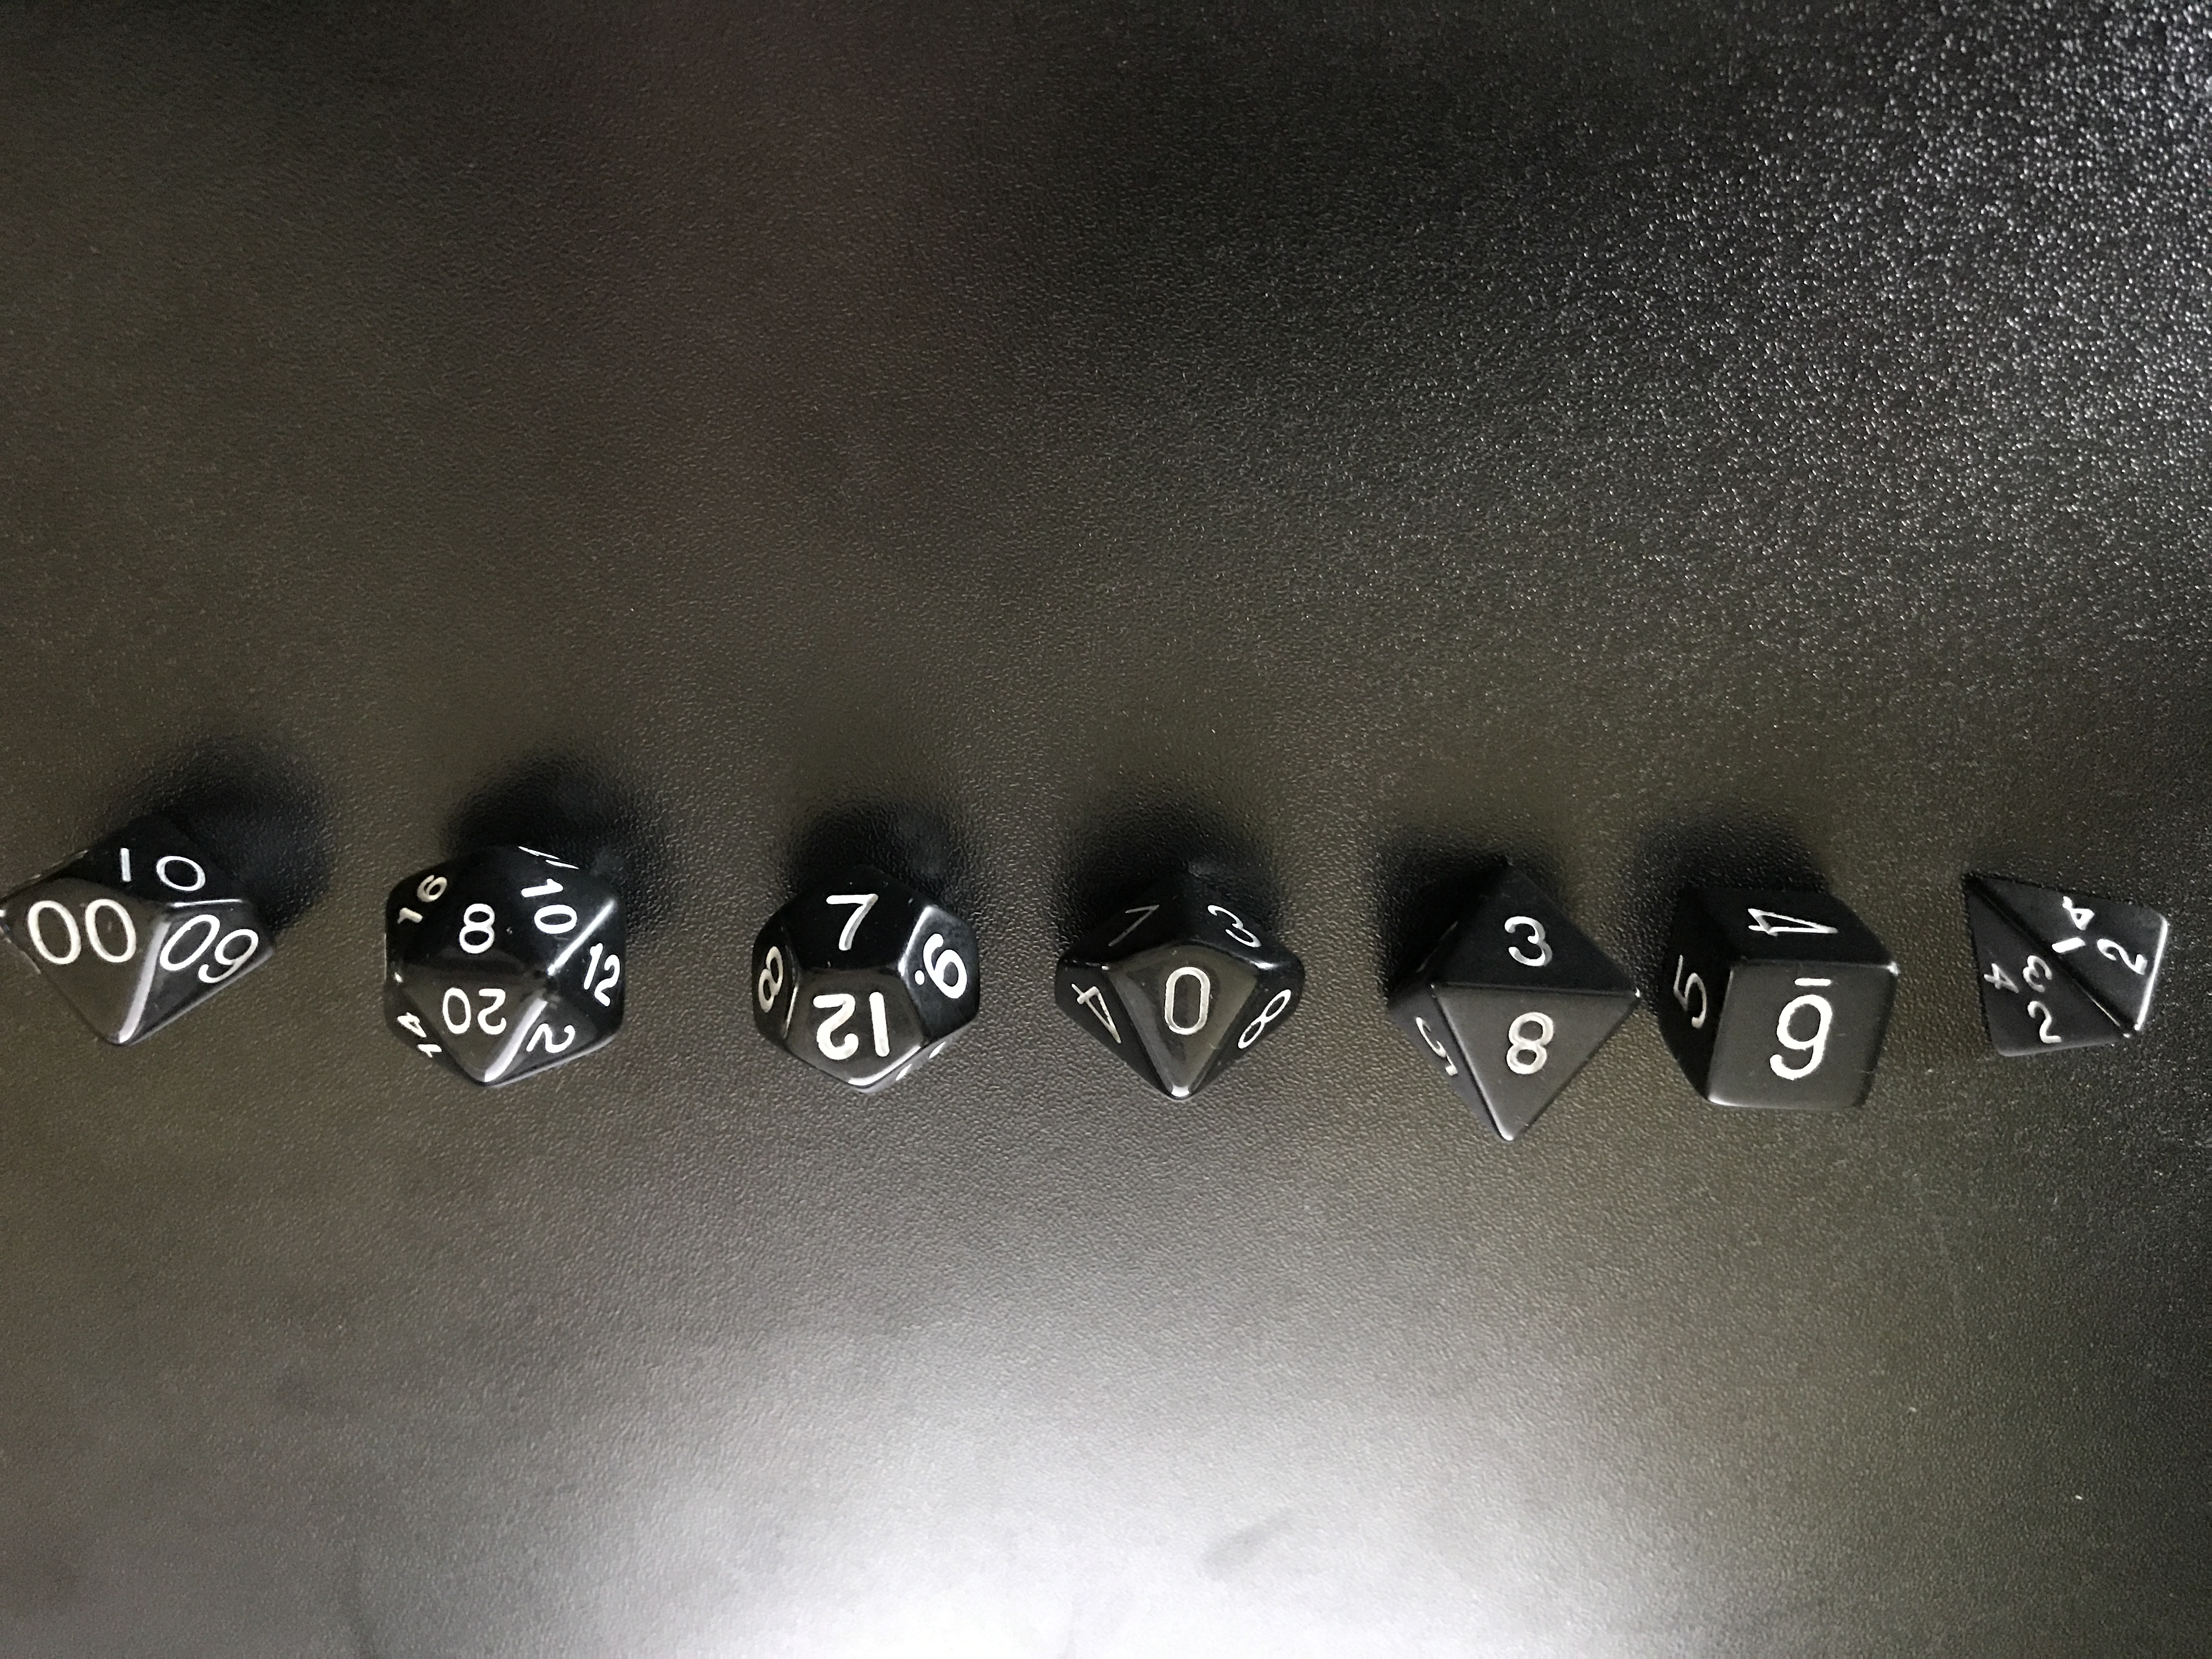
\includegraphics[width=1\linewidth, height=5cm, angle=180]{DnD_Dice.jpg}
			\label{DnDDice}
		\end{subfigure}
		\caption{(Left to Right) A: In this image we can see a typical \dnd \ table set up. The items on the table from left to right is the \emph{Monster Manual} \citep{MonsterManual}, scratch pad of paper, pens, series of die, DM's Screen, a battle mat, set of tokens, a character sheet, more die and the \emph{Player's Handbook} \citep{PlayerHandbook}. A group playing \dnd \ does not need all of the listed equipment each. The minimum equipment needed in a group, are the three core books (Player's Handbook, Monster Manual and \emph{Dungeon Master's Guide} \citep{DMGuide}), one set of die and some paper. Everything else is optional. \\ B: In this image we see the die necessary to play \dnd. They are (from left to right); 4, 6, 8, 10, 12, 20 and 100-sided. The die are denoted by the letter d followed by the number of sides (for example the 8-sided die is a d8). The d100 only has 10 sides but the sides increase in multiples of 10 and when rolled together with the d10 is known as the \emph{percentile die}.}
		\label{fig:DnDEquipmentExample}
	\end{figure}

	\subsection{Shortcomings of \dnd} \label{sec:shortcomings}
	\Codex \ is a system that will address some of the shortcomings within the 5\textsuperscript{th} Edition of \dnd. Whilst they are labelled as shortcomings they are integral to the game and there are not better alternatives. So rather than replacing these shortcomings, \Codex \ will attempt to fix them.
	
		\subsubsection{The Dungeon Master} \label{sec:DM}
		As explained in Appendix \ref{app:example}, the DM creates the world in front of the party and controls the narrative of the Campaign. Without a DM there can be no \dnd \ game. Therefore, the game of \dnd \ cannot survive without a healthy population of DMs.
		
		However, there is a great deal of pressure on the DM to create fun and engaging content for every single session of \dnd. The task of preparing content is time-consuming and often the work done by the DM can go unused. This commitment to a create content is off-putting to a lot of players who want to try their hand at running a game. The pressure put on a DM is no greater than during combat, as they have to track the individual statistics for each character in the battle in addition to maintaining the narrative.

		\subsubsection{\dnd \ is random} \label{sec:rand}
		In Appendix \ref{app:example} we saw the importance of die rolls in \dnd \ and the role of a DM. It is the die rolls that allows every game of \dnd \ to be unique and exciting. However, for the DM it the die rolls can cause of all their preparation work to be frequently wasted.
		
		\subsubsection{\dnd \ content is overlooked} \label{sec:overlooked}
		One of the most common questions a Player might ask a DM during a game is \emph{``Who was that guy back in that town from a couple of sessions ago?''}. Player's who do not take sufficient notes during a Campaign can often find themselves lacking in information when solving issues. Either the DM caves to the Player's request and digs out the information themselves, or the Party are stuck in the Campaign. 

	\subsection{Fixing the Shortcomings with \Codex} \label{sec:CodexFeatures}
	The features of \Codex \ are designed to solve the three shortcomings mentioned in Section \ref{sec:shortcomings}, the details of which will be discussed in Section \ref{sec:design}. \Codex \ will support the DM role by providing a platform for easy content creation. When a new \emph{Character} or \emph{Setting} is created within a Campaign, a ``Wikipedia'' style page will be generated. That both the Party and DMs can access. \Codex \ has a \emph{Combat Tracker} that will track combat statistics allowing the DM to focus on maintaining the narrative. 
		
		\subsubsection{Achieving \Codex} \label{sec:achieve}
		These features will be achieved through the use of the Agile Solo methodology \citep{AgileSolo}. Agile Solo is based to the Scrum Software Engineering Methodology \citep{Scrum}, which provides a system to track the development of a project and ensure that the deliverables are met. Scrum is developed for a team of people whereas Agile Solo is developed for single developer projects.
		
		The development of Codex will use the ReactJS and Node.JS JavaScript libraries. ReactJS can rapidly built and prototype User Interfaces (UI) across multiple platforms \citep{ReactJSOfficial}. Whilst, Node.JS will handle the passing of data between \Codex \ and the corresponding database \citep{NodejsOfficial}. Both of these technologies follow the basic Web-App Architecture laid out in Figure \ref{fig:web-app-arch}.
	
		\begin{figure}
			\centering
			\fbox{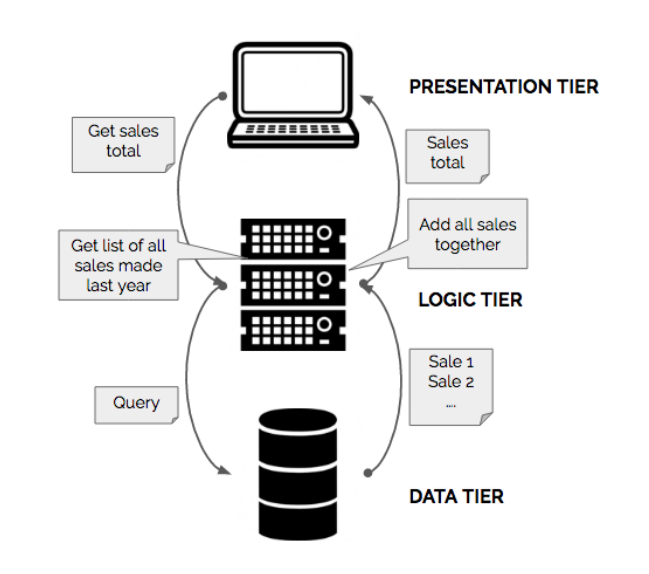
\includegraphics[width=0.5\textwidth]{Basic_Web_App_Architecture.PNG}} 
			\caption{Overview of a three-tier web application and its dependencies \citep{SecurityWebApps}. User Input is passed the Web-App through the Graphical User Interface (GUI) in the \emph{Presentation Tier} to the \emph{Logic Tier}. The \emph{Logic Tier} performs calculation on the data before passing it into the \emph{Data- Tier}. The \emph{Logic Tier} can also request data from the \emph{Data Tier}, to perform calculations, before passing the data back into the GUI to be displayed to the User.} \label{fig:web-app-arch}
		\end{figure}
	
	\section{\Codex \ Design} \label{sec:design}
	% Cherry pick sections from the Design Document, summarising how Codex is designed and why I made those choices.
	In this section, we will review the progress of the Design elements of \Codex. As we saw in Section \ref{sec:achieve}, \Codex \ following the Agile Solo methodology, which assists with maintaining project progress. Trello is used in conjunction with Agile Solo, see Figure \ref{fig:trello-board}, and requires a weekly review of the status of the project. Bi-weekly meetings with an external supervisor is also advised by Agile Solo.  
	
	\begin{figure}
		\centering
		\fbox{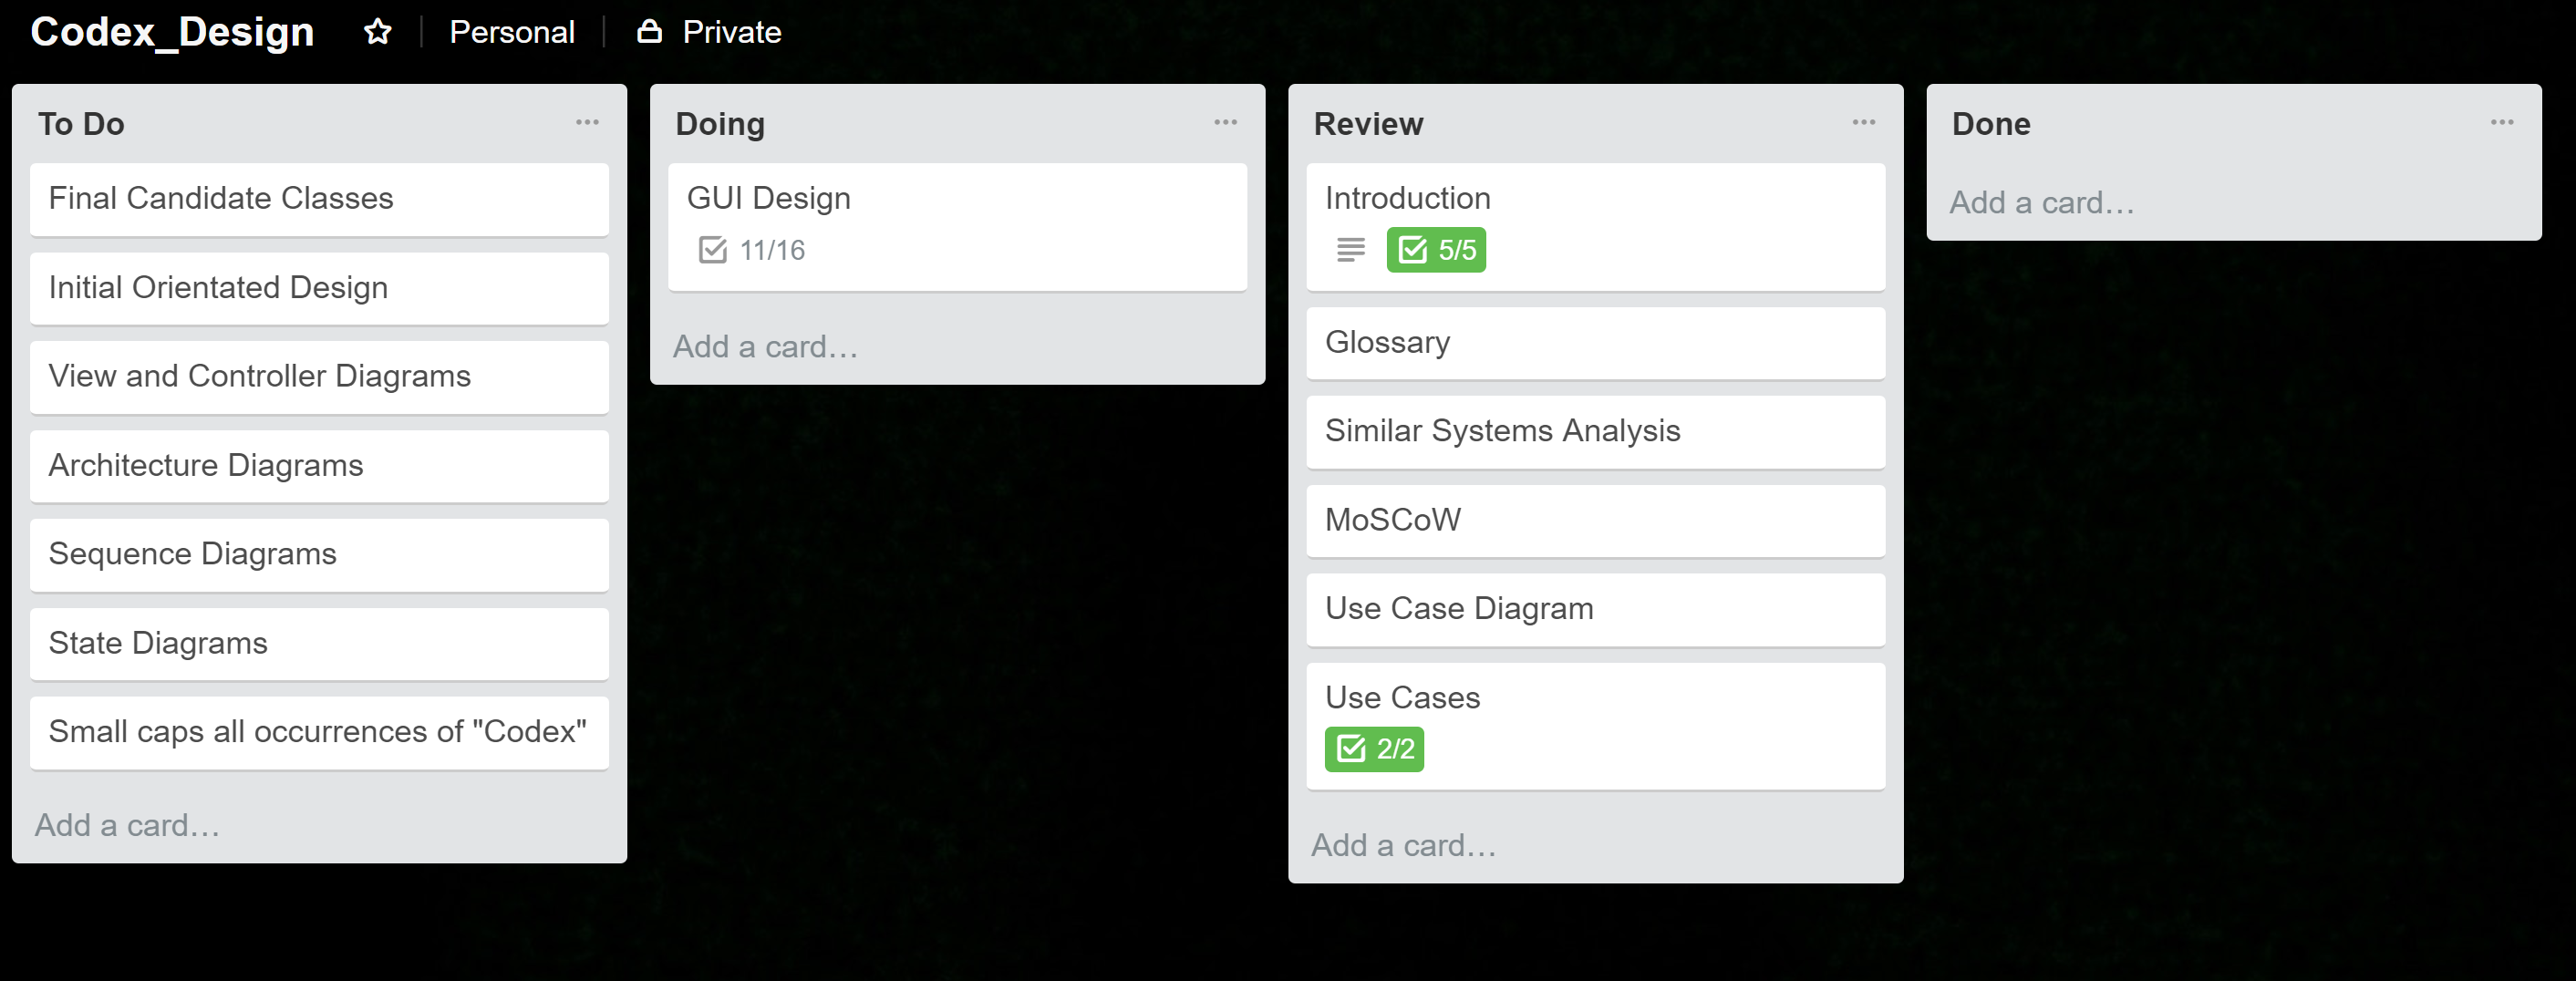
\includegraphics[width=0.5\textwidth]{trello_board.PNG}} 
		\caption{The Trello Board used to track the progress of the \Codex \ Design Iterations. Each item on Trello acts like a virtual post-it note. Each note containing a task that needs to be addressed.} \label{fig:trello-board}
	\end{figure}
	
		\subsection{Iterative Design} \label{sec:iterative}
		Agile Solo, see Sections \ref{sec:achieve} and \ref{sec:design}, supports an iterative form of development. The ReactJS JavaScript library complements iterative design due to the ability to rapidly prototype interfaces. However, before any development is performed, \Codex \ has passed through two phases of design. The first iteration focusing on low-fi prototyping (pen and paper) of the system, see Section \ref{sec:low-fi} . Think-Aloud Evaluations were then performed using the low-fi prototypes, with the feedback received incorporated into the second Development iteration, which focused on mid-fi prototyping (see Section \ref{sec:med-fi}) (using services such as the Marvel App \citep{marvelapp}).
	
		\subsection{The Use of ReactJS and Node.JS} \label{sec:languages}
		As discussed in section \ref{sec:achieve} and, \Codex \ aims to follow the Web-App Architecture displayed in Figure \ref{fig:web-app-arch}. The \emph{presentation} and \emph{logic} tiers will be built using ReactJS with the communication to and from the \emph{data} tier will be written in Node.JS (with the database itself written in SQL). In addition to providing a clear separation of languages and functionality the three-tier Web-App Architecture also follows the Model-View-Controller (MVC) architectural pattern \citep{ModelViewController}. However, the MVC architecture is complicated by the use of ReactJS, which blurs the line between the \emph{Model} (logic) and \emph{View} (presentation) tiers. This is a problem that will be addressed in Section \ref{sec:Issues}.
		
		\subsection{\Codex \ System Requirements} \label{sec:sys-req}
		The requirements for \Codex \ were generated by identifying the features that would solve the problems with \dnd \ that were discussed in Section \ref{sec:intro}. Once the features were generated, a \emph{MoSCoW Analysis} was performed on the list, see Table \ref{tab:MoSCoW} for the \Codex \ MoSCoW analysis.
		
		\begin{table}
			\centering
			\begin{tabular}{|c|c|c|c|}
				\hline
				\textbf{Must have} 					& \textbf{Should have}              	& \textbf{Could have} & \textbf{Won't have}             	  \\ \hhline{|=|=|=|=|}
				Track Combat      					&\makecell{Multiple Campaigns \\ per DM Account}	& \makecell{Game \\ Scheduling}     & \makecell{Full descriptions of \\ D\&D} \\ \hline
				Accounts          					& Settings								& Items               & \makecell{Pre-made Settings \\ \& Campaigns}\\ \hline
				Encounter Planning 					& Characters                        	&                     & \makecell{Inter-account Direct \\ Messaging} \\ \hline
				Random Encounters  					& WorldWiki                        		&                     &                                	  \\ \hline
				Populated Database 					& \makecell{Run, Save \& \\ Delete Games} 			&                     &                                   \\ \hline
				Session Planning					&         								&                     &                                   \\ \hline
			\end{tabular}
			\caption{MoSCoW analysis for \Codex, showing the differing importance of wanted features to the system as a whole. The \emph{Minimum Viable Product}(MVP) for the project is derived from the \emph{Must have} column. The \emph{Should have} column represents what features \Codex \ should contain for the system to be complete. The \emph{Could have} is what features might give \Codex \ an edge over similar systems and what would be ``nice to have''. Finally the \emph{Won't have} column represents what features will never be part of the \Codex \ system.}\label{tab:MoSCoW}
		\end{table}
	
		\subsection{Use Cases} \label{sec:use-cases}
		Another critical part of the Design of \Codex \ is planning how the functionality of the system will flow. \emph{Use Cases} and the \emph{Use Case Diagram } inform a developer how a data is expected to flow between systems during a function. See Figure \ref{fig:use-case-diag} for the \Codex \ Use Case Diagram. Each of the Use Cases listed in the Use Case Diagram is a single function within the \Codex \ system. The execution of each function is explained the corresponding Use Case, which the developer can refer to during development. Use Cases and Use Case Diagrams prevent errors and saves time during the development of a system.
		
		\begin{figure}[h]
			\centering
			\fbox{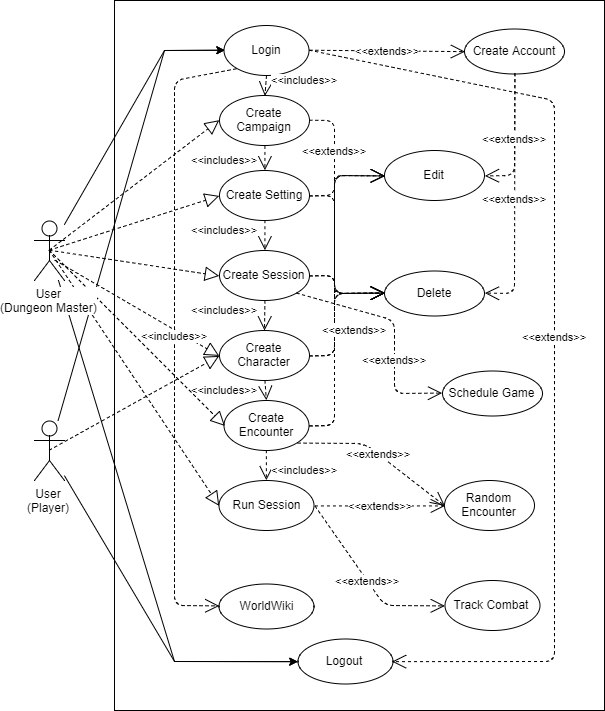
\includegraphics[width=0.5\textwidth]{use_case_diag.PNG}} 
			\caption{\Codex \ Use Case Diagram showing the accessibility to functions and the flow of information between them. Each node within the diagram is a Use Case and together explain how the various components of \Codex \ interact.} \label{fig:use-case-diag}
		\end{figure}
	
		\begin{figure}
			\centering
			\fbox{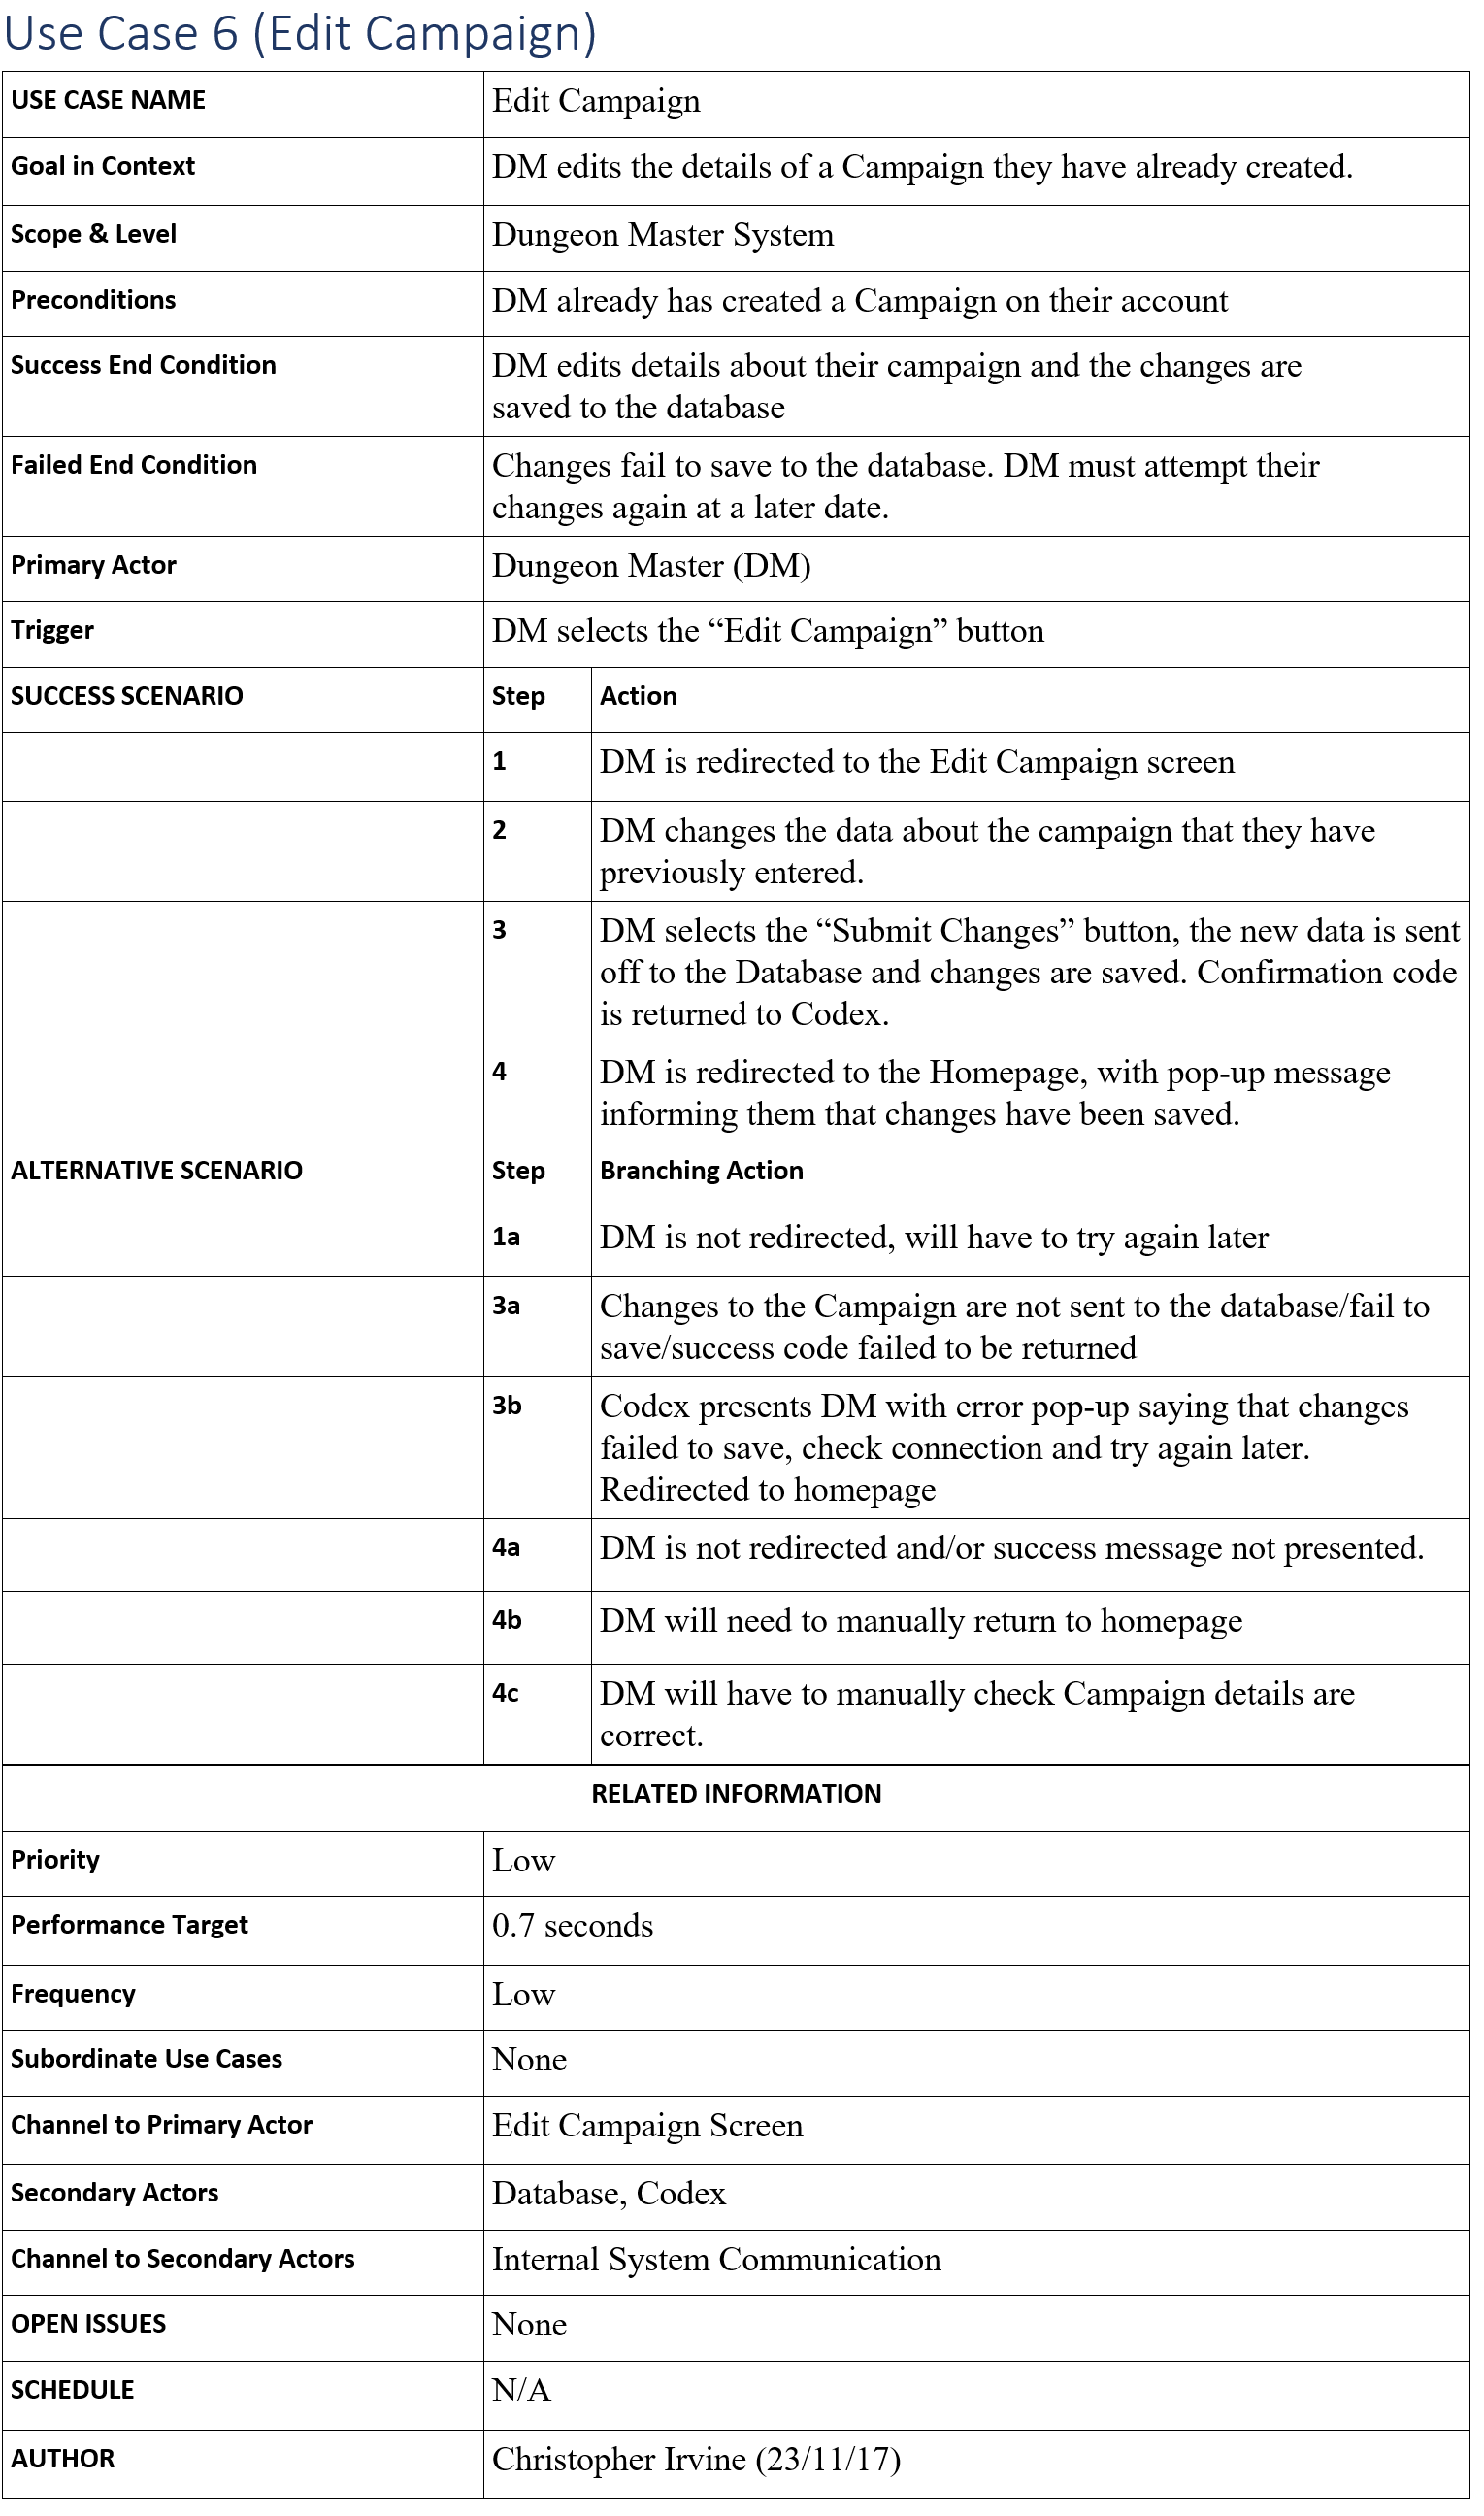
\includegraphics[width=0.75\textwidth]{use_case.PNG}}
			\caption{One of the Use Cases for \Codex, this is for Editing an existing Campaign. Use Cases provide details to the developer about how this function is expected to function, preventing error and saving time.}\label{fig:use-case}	
		\end{figure}
	
		\subsection{Low-Fi Prototyping} \label{sec:low-fi}
		Low-Fi Prototyping, as mentioned in Section \ref{sec:iterative} was used to test \Codex \ during the first iteration of Design. A low-fi prototype is a Pen and Paper sketch of what the GUI will look like. These sketches are then used in Think-Aloud Evaluations (where a subject is asked to vocalise their thoughts as they perform a series of tasks on a system) to ascertain the quality of the proposed GUI \citep{thinkaloud}. The GUI, initially, had several pop-up elements for the Editing and Deleting functions. 
		
		The subjects all reported the constant pop-ups as ``annoying'' and ``distracting''. During the second iteration of design the pop-up elements were minimised to system messages only, and were a lot less obtrusive.
	
		\subsection{Med-Fi Prototyping} \label{sec:med-fi}
		The Med-Fi prototypes were developed using MarvelApp \citep{marvelapp}, an online tool for the prototyping of system. Figure \ref{fig:med-fi} shows two example of the many med-fi screens that were developed. These med-fi screens are used during the development process (see Section \ref{sec:development}) as a guide for the developer to follow. Not only for how the system will appear to the user, but also how the screens will interact with each other. This process is also known as \emph{Wireframing}.
		
		\begin{figure}
			\begin{subfigure}{0.5\textwidth}
				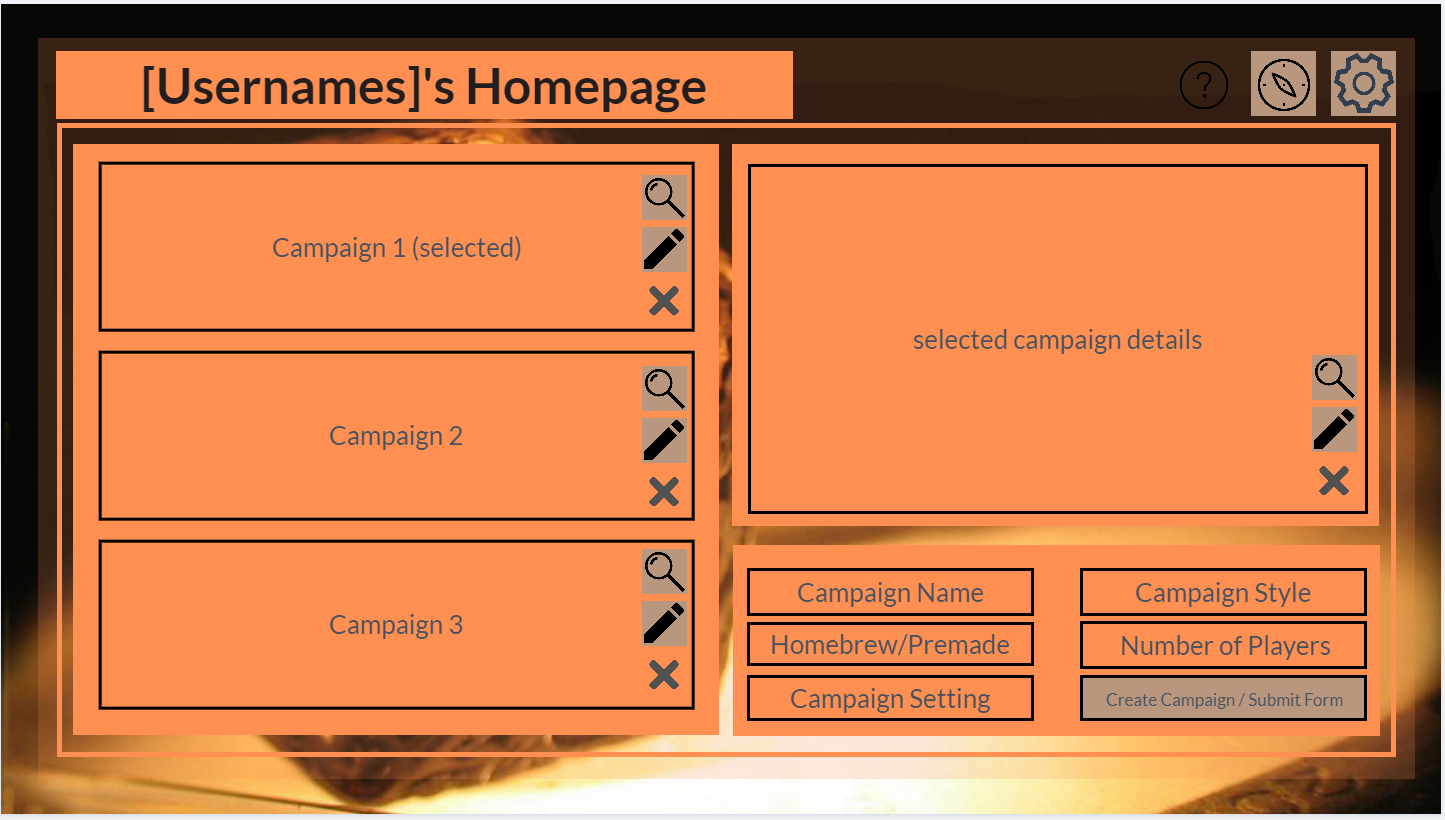
\includegraphics[width=1\linewidth, height=5cm]{homepage.png}
			\end{subfigure}
			\begin{subfigure}{0.5\textwidth}
				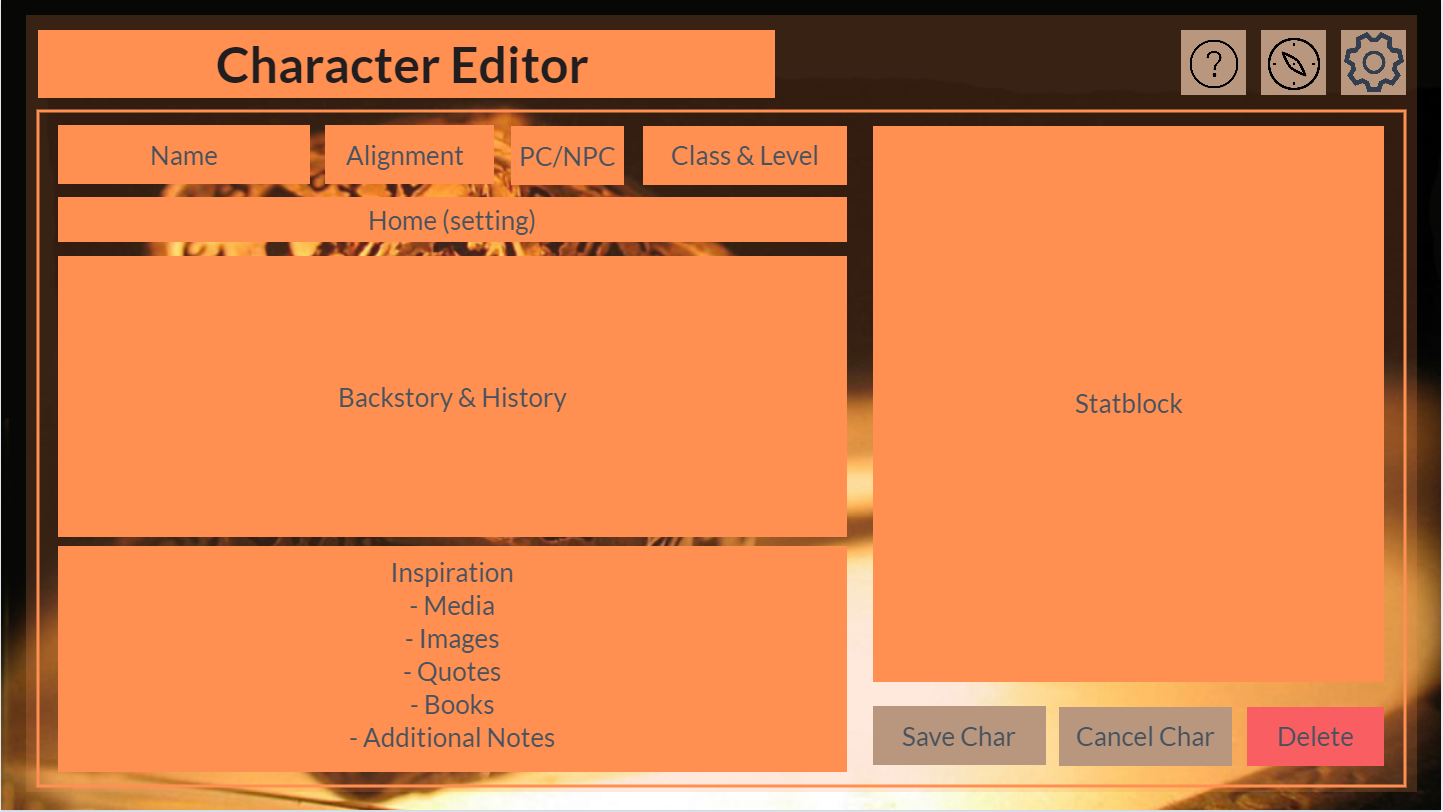
\includegraphics[width=1\linewidth, height=5cm]{character.png}
			\end{subfigure}
			\caption{(Left to Right)A: Med-Fi Prototype of the homepage, developed using MarvelApp. \\ B: Med-Fi Prototype of the Character Editor Screen, used in the Creation, Editing and Deletion of a Character. Developed using MarvelApp. \\ In both prototypes Navigation Elements can be seen along the top of the screen.}
			\label{fig:med-fi}
		\end{figure}
		
		\subsection{Object Orientated Design}
		An Object Orientated Design Diagram, like the other diagrams mentioned in Section \ref{sec:design}, provide guidance to a developer when programming a system. We can see in Figure \ref{fig:ood-views} the flow between the current containers predicted to be \Codex. Each container possess a series of a components. \Codex \ aims to reuse as many of these components between containers as possible. Additionally the Navigational Elements of the system will be a shared view. 
		
		\begin{figure}
			\centering
			\fbox{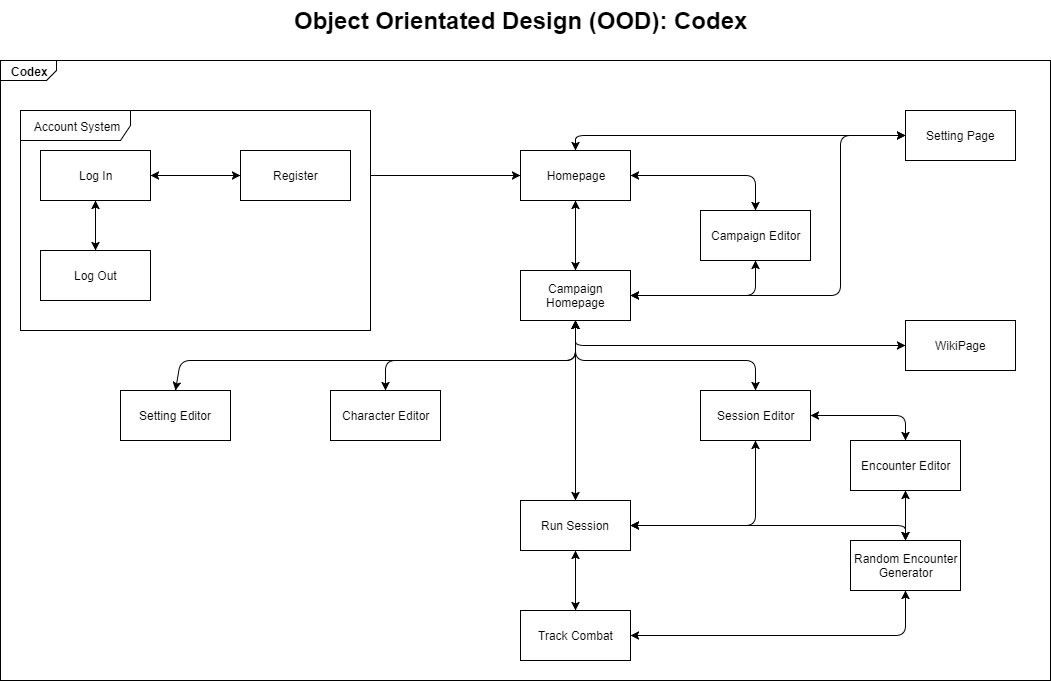
\includegraphics[width=0.75\textwidth]{Codex_View_OOD.PNG}} 
			\caption{Object Orientated Diagram for \Codex \ displaying the Container Components. Each container has a 1:1 relationship with each other. There is a subsystem present, called Account, that can be accessed through the Homepage regardless of the logged in state of the user.} \label{fig:ood-views}
		\end{figure}
	
	\section{\Codex \ Implementation Plan} \label{sec:development}
	In Section \ref{sec:design} we saw that several design elements for \Codex \ exist with the common goal of providing guidance for the development of \Codex. Figure \ref{fig:ood-views} and \ref{fig:use-case-diag} provide a ``road map'' for the development whilst Figures \ref{fig:use-case} and \ref{fig:med-fi} provide details of how the data flows between screens.
	
	The development of \Codex \ should now be able to progress at a faster pace because of the planning and considerations taken throughout the first two design iterations. It is expected that the design will further alter as the development progresses, when functions that were expected to occur in one way can only work in another.
	
	As discussed in Sections \ref{sec:achieve} and \ref{sec:iterative}, \Codex \ will be developed using the Agile Solo methodology. This will help the project stay on track through constant reviewing of already completed work and allowing the development to focus on one task at a time.
	
		\subsection{\Codex \ Gantt Chart} \label{sec:gantt}
		The initial Gantt Chart (see Appendix \ref{app:original}) generated for \Codex \ has changed slightly. The second design iteration of \Codex \ was brought forward in order to accommodate the Think-Aloud Evaluation results for the low-fi prototyping (see Section \ref{sec:low-fi}) before the development commenced. To compensate a Third Design Phase was added and the Development Iteration 1 was incorporated into Development Iteration 2. We should expect that the MVP for \Codex \ be completed by the end of Development Iteration 1 (see Appendix \ref{app:new}).
		
		\subsection{Language and Architecture} \label{sec:lang&arch}
		As we saw in Sections \ref{sec:languages} and \ref{sec:achieve} \Codex \ aims to use ReactJS in conjunction with Node.js in order to replicate a traditional Web-App Architecture (see Figure \ref{fig:web-app-arch}). The use of ReactJS, whilst providing a platform for rapid prototyping, testing and deployment, will also allow \Codex \ to be easily adapted for cross-platform use (iOS and Android). 
		
	\section{Outstanding Issues} \label{sec:Issues}
	% What are the issues with Codex? Are they being addressed? Any forthcoming issues?
	So far the progress of \Codex \ is satisfactory. There has not been a major delay or issue that \Codex \ has had to overcome. Minor issues do exist however. These are that \Codex \ has suffered from the needs of other university projects. Requiring time initially set aside for the development of \Codex \ be spent on these other projects. Additionally the Questionnaire mentioned in the Project Proposal has yet to be written or approved. 
	Outstanding Issues:

		\subsection{Solutions} \label{sec:solutions}
		In order to compensate for the lost development time the MVP for \Codex \ has been simplified to allow for faster development iterations. This also relieves the pressure from the developer so that the quality of the development remains high.
		
		The Questionnaire will be completed as part of Design Iteration 3 within the Gantt chart, however it will be written and approved as part of Development Iteration 1. By providing an extended period of time for the development of the Questionnaire and Ethics Approval, it increases the chance of the Questionnaire passing the Ethics Approval, as well as permitting time for adjustments to be made should it fail the Ethics Approval.
		
	\section{Conclusion} \label{sec:conclusions}
	% Summarise the progress that I have made, if it is enough and if not how can we do more?
	In this document; we have discussed the concepts of \dnd \ that is critical to \Codex, overlooked content, the DM and the random nature of \dnd \ (see Section \ref{sec:shortcomings}). Next we examined the current Design of \Codex, specifically examining the iterations \Codex \ has already gone through, the requirements \Codex \ must meet, use cases written to detail how the requirements will be achieved and the choice of languages (see Section \ref{sec:design}). Finally we reviewed the new Development Plan for \Codex \ and created Solutions for to handle the minor outstanding issues with the project (see Sections \ref{sec:development} and \ref{sec:Issues}).

	\clearpage
	\bibliography{projectbib}
	\appendix
	\section{Dungeons and Dragons Glossary} \label{app:example}
	\textbf{Player:} An individual who participates in a \textbf{Campaign} that is ran by a \textbf{Dungeon Master}. The player can either be a guest for a \textbf{session} or two, or a regular in the Campaign. Players control a \textbf{Player Character}. \\
	
	\textbf{Party:} A group of \textbf{Player Characters} that are allied with each other to achieve a common goal, usually the objective of the \textbf{Campaign}. Player Characters can join and leave the party at will, but typically \textbf{Players} will stay together for the duration of the Campaign that are playing through. \\ 
	
	\textbf{Dungeon Master (DM):} The individual who runs the game of Dungeons and Dragons for the \textbf{Players}. The role of a DM includes preparing content for each \textbf{session} of \dnd \ as well as narrate and control the sessions themselves.\\
	
	\textbf{Campaign:} A series of \textbf{challenges} that together form a story, known as the Campaign. The Campaign is created, prepared and ran by the \textbf{Dungeon Master}.\\
	
	\textbf{Setting:} \textbf{Campaigns} occur within a Setting. A Setting can be anything from a small fishing hamlet on the side of a lake to an entire planet or beyond. There can be multiple Settings within a Campaign. Usually, a DM will create their general Setting and populate it with more specific, smaller settings.\\
	
	\textbf{Sessions:} A Session is an episode within the Campaign that is delivered by the Dungeon Master to the Players, who react and interact with the session, which will impact the Campaign and in turn the Setting. Sessions need not be planned in detail, but do need guidelines, so that there is enough content for the Players to experience over the course of the session. \\
	
	\textbf{Character:} A fictional character within a \textbf{Setting} of Dungeons and Dragons. All characters have the same abilities, with different values. Characters are defined as \textbf{Player} or Non-Player. \\
	
	\textbf{Challenges:} A challenge is an obstacle that prevents the \textbf{Party} from progressing on with the \textbf{Campaign}. These challenges can be anything from persuading the Captain of a ship to give you passage, finding the entrance to a long lost ruined city or defeating an enemy in \textbf{Combat}. Challenges are resolved through \textbf{Die Rolls}. \\
	
	\textbf{Combat:} Combat is a physical altercation between the \textbf{Party} and a group of \textbf{Enemies}. Combat is over once one side has either fled or defeated the other. This is achieved by \textbf{Characters} attacking each other with \textbf{Attacks}, \textbf{Spells} and \textbf{Abilities}. \\
	
	\textbf{Spells/Abilities:} 	Spells/Abilities are powerful actions that a character can perform during the game. The number of times these can be performed is limited. Spells/Abilities can inflict \textbf{Damage} or \textbf{Healing} onto a target. \\
	
	\textbf{Attacks:} All Characters can make a number of Attacks with their action each turn. When an attack hits a target, All Characters can receive Healing, which restores lost HP. Unless stated otherwise, HP cannot be restored above the Maximum HP or applies to Temporary HP for the character. is inflicted. \\
	
	\textbf{Damage:} All Characters can receive Damage, when this happens that \textbf{Character} \textbf{Hit Points} drop an equal amount to damage received.\\
	
	\textbf{Healing:} All Characters can receive Healing, which restores lost \textbf{Hit Points}. \\
	
	\textbf{Hit Points (HP):} This represents how much damage a character can withstand before collapsing unconscious at 0 Hit Points. Characters have a Maximum limit to their Hit Points which increases when they grow stronger over time. Hit Points can be lost through \textbf{Damage} and restored \textbf{Healing}. \\
	
	\textbf{Proficiency:} When a \textbf{Character} is particularly skilled at a task, it is said they are \textit{Proficient} at it. When a character is Proficient they can apply a bonus \textit{Proficiency Modifier} to all rolls for that task. The proficiency modifier increases as characters get stronger. \\
	
	\textbf{Ability Statistics:} Every \textbf{Character} is defined by a set of six Ability Statistics \textit{(Strength, Dexterity, Constitution, Intelligence, Wisdom and Charisma)}. These can range from 0 to a potentially infinite amount, but usually the maximum is around 30. It is down to the preference of the \textbf{Dungeon Master}. \\
	
	\textbf{Ability Modifier:} The \textbf{Ability Statistics} translate into modifiers that can be applied to the relevant \textbf{Die Rolls}. This is done by taking the Ability Statistic, subtracting 10 and diving by 2 (then rounding up). This modifier can be positive or negative to reflect the strengths and weaknesses of each \textbf{character}. \\
	
	\textbf{Die Rolls:} All \textbf{challenges} in \dnd \ are resolved through Die Rolls. These are normally settled by rolling a 20-sided die (d20) and then applying the \textbf{Ability Modifier} and \textbf{Proficiency} to that die roll. The higher the result the more positive the outcome. 
	
	\textit{For example when Persuading a Guard for to give up information about the corrupt Baron who runs the town, would roll a Persuasion Roll. The character rolls a 11, a low result, but once he adds his Charisma (+4) and his Proficiency (for being Proficient in persuasion, +3) the roll is now 18. Which is likely more than enough to get some information out the guard.}
	
	\section{Gantt Chart - Original} \label{app:original}
	\begin{cmpfigure}{\Codex \ Gantt Chart, outlining the major tasks and deliverables\label{gc:original}}
		\begin{sideways}
			\newganttchartelement{voidbar}{
				voidbar/.style={draw=black, top color=black!25, bottom color=black!23
			}}
			\begin{ganttchart}[y unit chart = 0.86cm, y unit title = 0.86cm, x unit=0.35cm, vgrid, title label font=\scriptsize,
				canvas/.style={draw=black, dotted}]{1}{34}
				\gantttitle{Project schedule shown for e-vision week numbers
					and semester week numbers}{34} \\
				
				\gantttitlelist{8,...,41}{1}\\
				\gantttitlelist{1,...,12}{1} \gantttitle{CB}{4}
				\gantttitlelist{1,...,9}{1} \gantttitle{EB}{4}
				\gantttitlelist{10,...,14}{1}\\
				
				%The elements, bars and milestones, are identified as elem0, elem1, etc.
				\ganttbar{Project Proposal}{1}{2} \\        		%elem0  
				\ganttbar{Literature Review}{2}{5} \\      			%elem1 
				\ganttmilestone{Literature Review Finished}{5} \\	%elem2
				\ganttbar{Design Doc. Iteration 1}{4}{8} \\ 		%elem3
				\ganttbar{Development Iteration 1}{9}{11} \\		%elem4
				\ganttbar{Progress Report}{11}{12} 					%elem5
				\ganttmilestone{}{12} \\							%elem6
				\ganttbar{Development Iteration 2}{11}{12}  		%elem7
				%week 1 of semester 2 is the 17th week in schedule 
				\ganttvoidbar{}{13}{16} \\                     		%elem8
				\ganttbar{Final Report Writing 1}{17}{19} 	        %elem9
				\ganttmilestone{}{19} \\							%elem10
				\ganttbar{Design Doc. Iteration 2}{19}{20} \\      	%elem11
				\ganttbar{Development Iteration 3}{21}{26} \\		%elem12
				\ganttbar{Testing}{24}{26} \\						%elem13
				\ganttmilestone{Code Delivery}{26} \\       		%elem14
				\ganttbar{Final Report Writing 2}{27}{30} \\  		%elem15
				\ganttbar{Inspection preparation}{31}{34}   		%elem16
				
				\ganttlink{elem0}{elem1} \ganttlink{elem1}{elem2} \ganttlink{elem2}{elem3}
				\ganttlink{elem3}{elem4} \ganttlink{elem4}{elem5} \ganttlink{elem5}{elem6}
				\ganttlink{elem5}{elem7} \ganttlink{elem8}{elem9} \ganttlink{elem10}{elem11}
				\ganttlink{elem11}{elem12} \ganttlink{elem12}{elem13} 
				\ganttlink{elem13}{elem14} \ganttlink{elem14}{elem15}
				\ganttlink{elem15}{elem16}
			\end{ganttchart}
		\end{sideways}
	\end{cmpfigure}

	\section{Gantt Chart - New} \label{app:new}
	\begin{cmpfigure}{Revised \Codex \ Gantt Chart, outlining the major tasks and deliverables\label{gc:new}}
		\begin{sideways}
			\newganttchartelement{voidbar}{
				voidbar/.style={draw=black, top color=black!25, bottom color=black!23
			}}
			\begin{ganttchart}[y unit chart = 0.86cm, y unit title = 0.86cm, x unit=0.35cm, vgrid, title label font=\scriptsize,
				canvas/.style={draw=black, dotted}]{1}{34}
				\gantttitle{Project schedule shown for e-vision week numbers
					and semester week numbers}{34} \\
				
				\gantttitlelist{8,...,41}{1}\\
				\gantttitlelist{1,...,12}{1} \gantttitle{CB}{4}
				\gantttitlelist{1,...,9}{1} \gantttitle{EB}{4}
				\gantttitlelist{10,...,14}{1}\\
				
				%The elements, bars and milestones, are identified as elem0, elem1, etc.
				\ganttbar{Project Proposal}{1}{2} \\        		%elem0  
				\ganttbar{Literature Review}{2}{5} \\      			%elem1 
				\ganttmilestone{Literature Review Finished}{5} \\	%elem2
				\ganttbar{Design Doc. Iteration 1}{4}{8} \\ 		%elem3
				\ganttbar{Design Doc. Iteration 2}{9}{11} \\		%elem4
				\ganttbar{Progress Report}{11}{12} 					%elem5
				\ganttmilestone{}{12} \\							%elem6
				\ganttbar{Development Iteration 1}{13}{17} \\  		%elem7
				%week 1 of semester 2 is the 17th week in schedule 
				\ganttbar{Final Report Writing 1}{17}{19} 	        %elem8
				\ganttmilestone{}{19} \\							%elem9
				\ganttbar{Design Doc. Iteration 3}{19}{20} \\      	%elem10
				\ganttbar{Development Iteration 2}{21}{26} \\		%elem11
				\ganttbar{Testing}{24}{26} \\						%elem12
				\ganttmilestone{Code Delivery}{26} \\       		%elem13
				\ganttbar{Final Report Writing 2}{27}{30} \\  		%elem14
				\ganttbar{Inspection preparation}{31}{34}   		%elem15
				
				\ganttlink{elem0}{elem1} \ganttlink{elem1}{elem2} \ganttlink{elem2}{elem3}
				\ganttlink{elem3}{elem4} \ganttlink{elem4}{elem5} \ganttlink{elem5}{elem6}
				\ganttlink{elem5}{elem7} \ganttlink{elem7}{elem8} \ganttlink{elem9}{elem10}
				\ganttlink{elem10}{elem11} \ganttlink{elem11}{elem12} 
				\ganttlink{elem12}{elem13} \ganttlink{elem13}{elem14} 
				\ganttlink{elem14}{elem15}
			\end{ganttchart}
		\end{sideways}
	\end{cmpfigure}
	

\end{document}
% EOF Document